\documentclass[aspectratio=169]{beamer}

% ---------------- Packages ----------------
\usepackage{amsmath, amssymb, mathtools}
\usepackage{tikz}
\usetikzlibrary{arrows.meta, positioning, shapes, calc}
\usepackage{hyperref}

% ---------------- Theme ----------------
\usetheme{Madrid}
\usecolortheme{default}
\setbeamertemplate{navigation symbols}{}

% ---------------- TikZ Styles ----------------
\tikzset{
  node/.style={draw, rectangle, rounded corners, minimum width=2cm, minimum height=0.8cm},
  source/.style={node, fill=red!15},
  sink/.style={node, fill=blue!15},
  entity/.style={node, fill=gray!10},
  taint/.style={->, thick, red},
  flow/.style={->, thick},
}

% ---------------- Metadata ----------------
\title{Taint Analysis via CFL-Reachability}
\author{Mostafa Hassanein}
\date{03, January 2026}

\begin{document}

% ============================================================
\begin{frame}
  \titlepage
\end{frame}

% ============================================================
\begin{frame}{Agenda}
\begin{itemize}
  \item<1-> What is taint analysis?
  \item<2-> Why is it important?
  \item<3-> Why context sensitivity is needed?
  \item<4-> CFL-reachability formulation
  \item<5-> Examples
\end{itemize}
\end{frame}

% ============================================================
\begin{frame}{Static Analysis}
\begin{itemize}
  \item<1-> Static analysis reasons about \emph{all executions} without running the program
  \item<2-> It computes a sound over-approximation of behaviors
  \item<3-> Taint analysis is a data-flow–based static analysis
\end{itemize}
\end{frame}

% ============================================================
\begin{frame}{What Is Taint Analysis?}
\begin{itemize}
  \item<1-> Tracks flow of untrusted (tainted) data
  \item<2-> Detects whether tainted data reaches sensitive operations
  \item<3-> Abstracts away concrete values, tracking dependencies
\end{itemize}

\medskip
\onslide<4->{
\textbf{Core Question:}
\begin{quote}
Does tainted data flow from a source to a sink along a valid execution?
\end{quote}
}
\end{frame}

% ============================================================
\begin{frame}{Example: SQL Query Template}
\begin{block}{Intended Query}
\texttt{
SELECT balance \\
FROM AcctData \\
WHERE name = ':n' AND password = ':p'
}
\end{block}
\end{frame}

% ============================================================
\begin{frame}{Malicious User Input}
\onslide<1->{
\[
n = \texttt{``Charles Dickens' --''}
\quad
p = \texttt{``who cares''}
\]
}

\onslide<2->{
\begin{block}{Resulting Query}
\texttt{
SELECT balance FROM AcctData \\
WHERE name = 'Charles Dickens' --' \\
AND password = 'who cares'
}
\end{block}
}

\begin{itemize}
  \item<3-> Password check is commented out
  \item<4-> Sensitive data is leaked
\end{itemize}
\end{frame}

% ============================================================
\begin{frame}{Taint Propagation Graph}
\centering
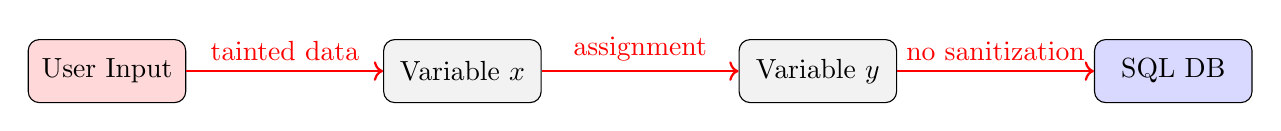
\begin{tikzpicture}[node distance=2.5cm]
  \node[source] (src) {User Input};
  \node[entity, right=of src] (x) {Variable $x$};
  \node[entity, right=of x] (y) {Variable $y$};
  \node[sink, right=of y] (db) {SQL DB};

  \draw[taint] (src) -- node[above]{tainted data} (x);
  \draw[taint] (x) -- node[above]{assignment} (y);
  \draw[taint] (y) -- node[above]{no sanitization} (db);
\end{tikzpicture}

\medskip
\begin{itemize}
  \item<2-> Nodes represent program entities (variables or functions)
  \item<3-> Edges represent labeled data-flow relations
\end{itemize}
\end{frame}

% ============================================================
\begin{frame}{Why Context Sensitivity Is Needed}
\begin{itemize}
  \item<1-> The same function may be called from different sites
  \item<2-> Taint behavior depends on the calling context
  \item<3-> Context-insensitive analysis merges incompatible flows
\end{itemize}
\end{frame}

% ============================================================
\begin{frame}{Context-Insensitive Call Graph}
\centering
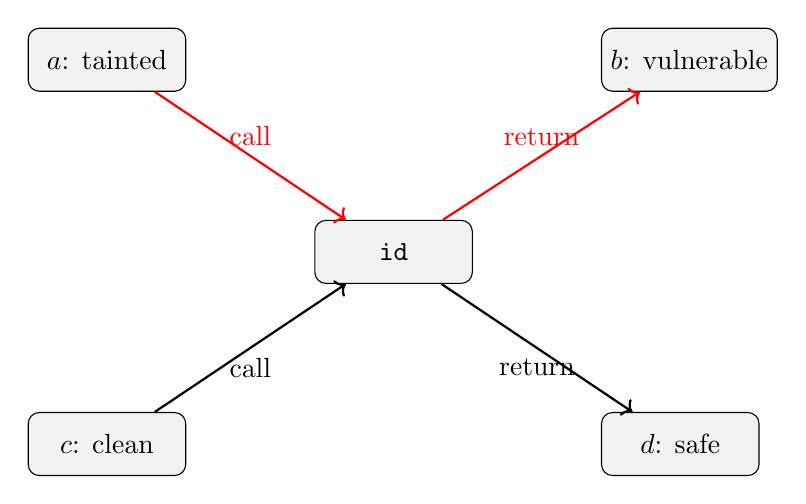
\begin{tikzpicture}[node distance=2.3cm]
  \node[entity] (id) {\texttt{id}};
  \node[entity, above left=of id] (a) {$a$: tainted};
  \node[entity, below left=of id] (c) {$c$: clean};
  \node[entity, above right=of id] (b) {$b$: vulnerable};
  \node[entity, below right=of id] (d) {$d$: safe};

  \draw[taint] (a) -- node[above]{call} (id);
  \draw[flow] (c) -- node[below]{call} (id);
  \draw[taint] (id) -- node[above]{return} (b);
  \draw[flow] (id) -- node[below]{return} (d);
\end{tikzpicture}

\medskip
\onslide<2->{
\textbf{Spurious taint flow appears due to context merging.}
}
\end{frame}

% ============================================================
\begin{frame}{Invalid Reachability Path}
\begin{itemize}
  \item<1-> Clean call enters function
  \item<2-> Tainted return exits function
  \item<3-> Path exists in graph but not in execution
\end{itemize}

\medskip
\onslide<4->{
\[
\text{call}_{\text{clean}} \;\; \text{return}_{\text{tainted}}
\quad \text{(invalid)}
\]
}
\end{frame}

% ============================================================
\begin{frame}{Program Graph Model}
\onslide<1->{
A program is modeled as a labeled graph
\[
G = (V, E, \Sigma)
\]
}

\begin{itemize}
  \item<2-> $V$: program entities
  \item<3-> $E \subseteq V \times \Sigma \times V$: labeled edges
  \item<4-> $\Sigma$: flow actions (call, return, assign)
\end{itemize}
\end{frame}

% ============================================================
\begin{frame}{Paths and Labels}
\onslide<1->{
A path
\[
\pi = v_0 \xrightarrow{a_1} v_1 \xrightarrow{a_2} \cdots \xrightarrow{a_k} v_k
\]
}

\onslide<2->{
induces a word
\[
\ell(\pi) = a_1 a_2 \cdots a_k
\]
}

\medskip
\onslide<3->{
Only some words correspond to valid executions.
}
\end{frame}

% ============================================================
\begin{frame}{Grammar for Valid Taint Flows}
\onslide<1->{
\[
F \;\rightarrow\; FF 
\;\mid\; call_i \; F \; return_i
\;\mid\; assign
\;\mid\; \varepsilon
\]
}

\begin{itemize}
  \item<2-> $call_i / return_i$: Procedure invocation and return matching call site $i$
  \item<3-> \texttt{assign}: Local data flow within a procedure
  \item<4-> \textbf{Result:} Only matching pairs $(call_i, return_i)$ are derivable. This filters out paths that do not correspond to feasible call stacks.
\end{itemize}
\end{frame}

% ============================================================
\begin{frame}{Taint Analysis as CFL-Reachability}
\onslide<1->{
\begin{block}{Problem}
Given $s,t \in V$, does there exist a path $\pi$ from $s$ to $t$ such that
\[
\ell(\pi) \in L(\mathcal{G})?
\]
\end{block}
}

\onslide<2->{
This exactly captures context-sensitive taint analysis.
}
\end{frame}

% ============================================================
% =================== WORKED EXAMPLES ========================
% ============================================================

\begin{frame}{Example 1: The Identity Crisis (Context Matching)}

\centering
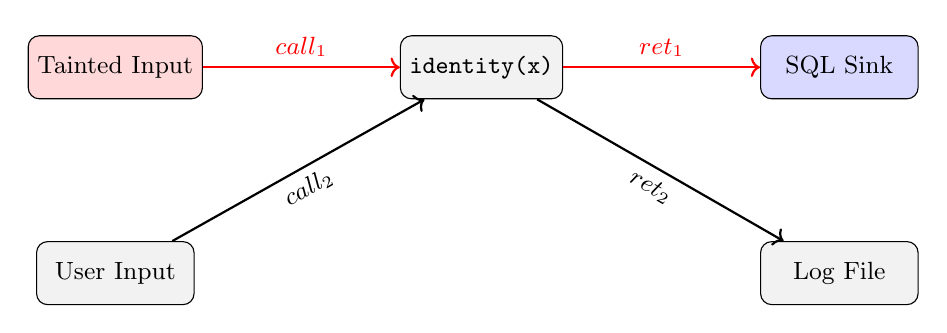
\begin{tikzpicture}[node distance=1.8cm, font=\small]
  \node[source] (src) {Tainted Input};
  \node[entity, below=of src] (clean) {User Input};
  \node[entity, right=2.5cm of src] (id) {\texttt{identity(x)}};
  \node[sink, right=2.5cm of id] (sink) {SQL Sink};
  \node[entity, below=of sink] (safe) {Log File};

  \draw[taint] (src) -- node[above, sloped]{$call_1$} (id);
  \draw[flow] (clean) -- node[below, sloped]{$call_2$} (id);
  
  \draw[taint] (id) -- node[above, sloped]{$ret_1$} (sink);
  \draw[flow] (id) -- node[below, sloped]{$ret_2$} (safe);
\end{tikzpicture}

\medskip
\begin{itemize}
    \item<2-> \textbf{Graph Path:} A path exists from \textit{Tainted Input} to \textit{Log File} via $call_1 \to ret_2$.
    \item<3-> \textbf{CFL Check:} $call_1 ret_2$ is \textbf{not} in $L(\mathcal{G})$ because indices 1 and 2 don't match.
    \item<4-> \textbf{Insight:} Grammar prevents tainted data from "leaking" into different call sites.
\end{itemize}
\end{frame}

% ============================================================
\begin{frame}{Example 2: Deep Recursion (Self-Referential Flow)}

\centering
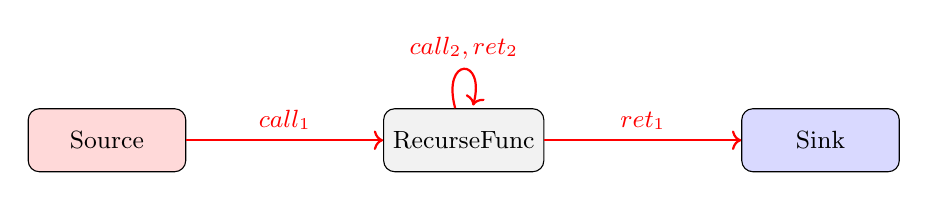
\begin{tikzpicture}[node distance=2.5cm, font=\small]
  \node[source] (s) {Source};
  \node[entity, right=of s] (rec) {RecurseFunc};
  \node[sink, right=of rec] (sink) {Sink};

  \draw[taint] (s) -- node[above]{$call_1$} (rec);
  
  % Self-loop representing recursion
  \draw[taint] (rec) edge [loop above] node {$call_2, ret_2$} (rec);
  
  \draw[taint] (rec) -- node[above]{$ret_1$} (sink);
\end{tikzpicture}

\medskip
\begin{itemize}
    \item<2-> \textbf{Scenario:} A function calls itself. Taint flows through an arbitrary number of recursive steps.
    \item<3-> \textbf{Word:} $\ell(\pi) = call_1 (call_2)^n (ret_2)^n ret_1$.
    \item<4-> \textbf{CFL Validation:} This is a classic $a^n b^n$ structure. The grammar $F \to call_i F ret_i$ naturally accepts balanced recursive calls, ensuring the data eventually returns to the correct caller.
\end{itemize}
\end{frame}

% ============================================================
\begin{frame}{Example 3: Sanitization Logic (Path Selection)}

\centering
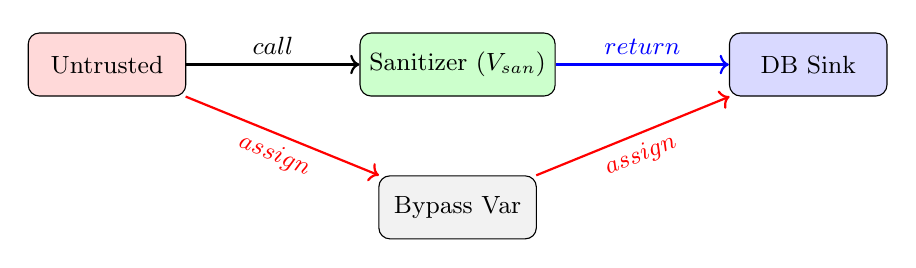
\begin{tikzpicture}[node distance=2.2cm, font=\small]
  \node[source] (src) {Untrusted};
  \node[entity, right=of src, fill=green!20] (san) {Sanitizer ($V_{san}$)};
  \node[sink, right=of san] (sink) {DB Sink};
  \node[entity, below=1cm of san] (bypass) {Bypass Var};

  \draw[flow] (src) -- node[above]{$call$} (san);
  \draw[flow, blue] (san) -- node[above]{$return$} (sink);
  \draw[taint] (src) -- node[below, sloped]{$assign$} (bypass);
  \draw[taint] (bypass) -- node[below, sloped]{$assign$} (sink);
\end{tikzpicture}

\medskip
\begin{itemize}
    \item<1-> \textbf{Formal Condition:} A path $\pi$ is a violation if $\ell(\pi) \in L(\mathcal{G})$ and $V(\pi) \cap V_{san} = \emptyset$.
    \item<2-> \textbf{Sanitized Path:} $\pi_{top} = (\text{Untrusted} \to \text{Sanitizer} \to \text{Sink})$. 
    Since $\text{Sanitizer} \in V_{san}$, this path is \textbf{discarded} despite being in $L(\mathcal{G})$.
    \item<3-> \textbf{Vulnerable Path:} $\pi_{bot} = (\text{Untrusted} \to \text{Bypass} \to \text{Sink})$.
    $\ell(\pi_{bot}) = assign \cdot assign \in L(\mathcal{G})$ and avoids $V_{san}$. \textbf{Violation detected.}
\end{itemize}
\end{frame}

% ============================================================
\begin{frame}{Summary}
\begin{itemize}
  \item<1-> Taint analysis tracks information flow
  \item<2-> Context insensitivity yields false positives
  \item<3-> Valid executions form a context-free language
  \item<4-> CFL-reachability provides principled context sensitivity
\end{itemize}
\end{frame}

% ============================================================
\begin{frame}{References}
\small
\begin{itemize}
  \item Aho, Alfred V., et al. Compilers: Principles, Techniques, and Tools. 2nd ed., Pearson Education, 2006.
\end{itemize}
\end{frame}

% ============================================================
\begin{frame}
\centering
\Large Thank you \\
\vspace{1cm}
\small \textit{Questions?}
\end{frame}

\end{document}